\documentclass[a4paper]{article}
\usepackage[utf8]{inputenc}
\usepackage[margin=1in]{geometry}
\usepackage{wrapfig}
\usepackage{graphicx}
\usepackage{enumitem}

\title{Induction Exercises}
\author{Ben Kettle - Adapted from MIT 8.02}
\date{22 January 2020}

\begin{document}

\maketitle

\section{Falling Loop}

\begin{wrapfigure}{r}{0.34\textwidth}
  \begin{center}
    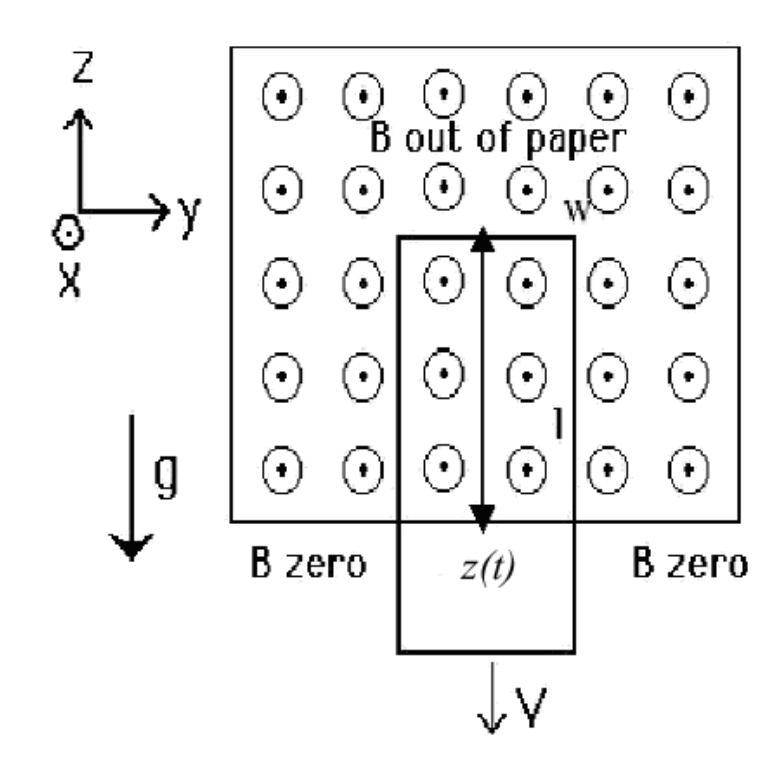
\includegraphics[width=0.3\textwidth,trim={0 5mm 0 10mm}, clip]{ex1fig.png}
  \end{center}
\end{wrapfigure}

Suppose a rectangular loop with mass $m$, width $w$, vertical length $l$, and resistance $R$ is falling out of a magnetic field under the influence of gravity. The magnetic field is uniform and out of the page ($\vec{B} = B\hat{x}$) within the area shown and zero outside of that area. The loop is exiting the magnetic field with $\vec{V}(t) = V(t)\hat{z}$, where $V(t) < 0$ (the loop is moving downward). Define the distance from the top of the loop to the bottom of the magnetic field at time $t$ as $z(t)$.

\begin{enumerate}[label=(\alph*), itemsep=9.8mm]
    \item What is the relationship between the distance $z(t)$ and the speed $V(t)$? Remember that $z(t)$ is positive and decreasing in time, and $V(t)$ is negative.
    \item If we define the area vector $\vec{A}$ to be out of the page, what is the magnetic flux $\Phi_B$ through the circuit at time $t$ (in terms of $z(t)$, not $V(t)$.).
\end{enumerate}

\begin{enumerate}[label=(\alph*), itemsep=9.8mm,topsep=9.8mm]
    \setcounter{enumi}{3}
    \item Find $d\Phi_B/dt$. Is it positive or negative at time $t$? Your answer should include $V(t)$.
    \item What is the direction of the induced current in the loop?
    \item What is the direction of the magnetic field created by this current? 
    \item What is the magnitude of the current flowing in the circuit at the time $t$?
    \item What other force (besides gravity) is acting on the loop in the $\pm \hat{z}$ direction? Give the magnitude and direction of this force in terms of the quantities given.
    \item Assume the loop has reached terminal velocity---it is no longer accelerating. What is the magnitude of that terminal velocity in terms of the given quantities?
 \end{enumerate}
 
\section{Power Transmission}
You've started a new job at the electric company, and want to determine the best way to send power across Ancona. The stretch of power lines you are working with has a total resistance of $.40 \Omega$, and the solar panels you are using as a power source generate $240V$ power. On average, $120 kW$ of power is sent through the lines. You are considering using a transformer, and want to minimize power loss during transmission. 

\begin{enumerate}[label=(\alph*), itemsep=9.8mm,after=\vspace{9.8mm}]
\item Calculate the power loss over the length of the transmission lines without the transformer.

\item Calculate the power loss through the transmission lines with a transformer added between the solar panels and the transmission lines. The transformer has 10 primary (input) turns and 1,000 secondary (output) turns.

\item Should you use the transformer in this case? How could you decrease power loss further?

\end{enumerate}

\section{Circuit Concepts}
A circuit consists of two resistors $R_1$ and $R_2$, a capacitor, and a switch. The switch has been open for a very long time and is closed at $t=0$.
\begin{enumerate}[itemsep=4mm,after=\vspace{4mm}]
    \item What is the current through the capacitor at $t=0^+$, just after the switch is closed?
    \item What are the currents through $R_1$ and $R_2$ at $t=0^+$?
    \item What is the current through the capacitor at $t = \infty$?
    \item What are the currents through $R_1$ and $R_2$ at $t=\infty$?
\end{enumerate}

\section{Purely Resistive Circuit}
\begin{figure}[h]
    \centering
    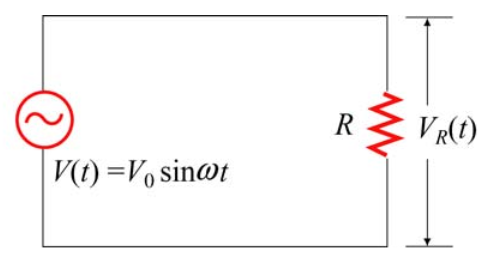
\includegraphics[scale=.5]{resistorcircuit.png}
    \label{fig:resistorcircuit}
\end{figure}

Recall that for AC Circuits, we define $V(t) = V_0 sin(\omega t)$ and $I(t) = I_0 sin(\omega t - \phi)$. The above circuit consists of an AC voltage source with voltage defined by $V(t) = V_0 sin(\omega t)$ and a resistor with resistance $R$. 

\begin{enumerate}[label=(\alph*), itemsep=5mm,after=\vspace{5mm}]
    \item Use Kirchoff's loop rule to find the circuit equation.
    \item Find the values of $I_0$ and $\phi$ for this circuit.
    \item Find the room-mean-squared power $P_{rms}$ disappated by this circuit. Recall that $\frac{1}{T}\int_0^T sin^2(t) = \frac{1}{2}$.
\end{enumerate}

\section{Purely Inductive Circuit}
    \begin{figure}[h]
        \centering
        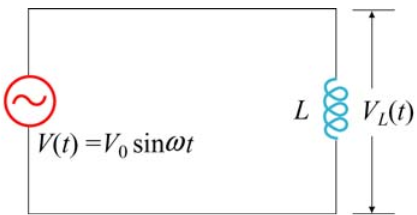
\includegraphics[scale=.5]{inductorcircuit.png}
        \label{fig:inductorcircuit}
    \end{figure}
    
Now, the same voltage source with $V(t) = V_0 sin(\omega t)$ is connected to an inductor with inductance $L$. 
\begin{enumerate}[label=(\alph*), itemsep=5mm,after=\vspace{5mm}]
    \item Use Kirchoff's loop rule to find the circuit equation.
    \item For current in the form $I(t) = I_0 sin(\omega t - \phi)$, find the values of $I_0$ and $\phi$ for this circuit.
\end{enumerate}

\section{Purely Capacative Circuit}
    \begin{figure}[h]
        \centering
        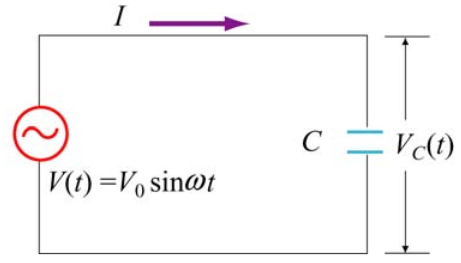
\includegraphics[scale=.5]{capacitorcircuit.png}
        \label{fig:capacitorcircuit}
    \end{figure}
    Finally, the same voltage source is connected to only a capacitor. Once again, voltage is given by $V(t) = V_0 sin(\omega t)$.
    \begin{enumerate}[label=(\alph*), itemsep=5mm,after=\vspace{5mm}]
    \item Use Kirchoff's loop rule to find the circuit equation.
    \item For current in the form $I(t) = I_0 sin(\omega t - \phi)$, find the values of $I_0$ and $\phi$ for this circuit.
\end{enumerate}

\end{document}